% Created by tikzDevice version 0.10.1 on 2016-06-30 12:57:10
% !TEX encoding = UTF-8 Unicode
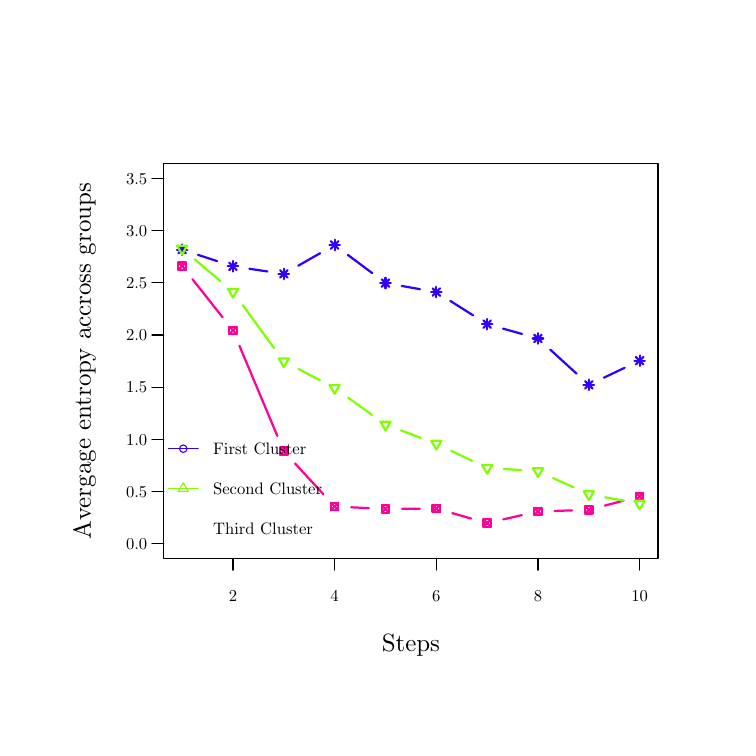
\begin{tikzpicture}[x=1pt,y=1pt]
\definecolor{fillColor}{RGB}{255,255,255}
\path[use as bounding box,fill=fillColor,fill opacity=0.00] (0,0) rectangle (252.94,252.94);
\begin{scope}
\path[clip] ( 49.20, 61.20) rectangle (227.75,203.75);
\definecolor{drawColor}{RGB}{51,0,255}

\path[draw=drawColor,line width= 0.8pt,line join=round,line cap=round] ( 61.52,170.85) -- ( 68.48,168.58);

\path[draw=drawColor,line width= 0.8pt,line join=round,line cap=round] ( 80.12,165.82) -- ( 86.62,164.85);

\path[draw=drawColor,line width= 0.8pt,line join=round,line cap=round] ( 97.77,166.93) -- (105.70,171.44);

\path[draw=drawColor,line width= 0.8pt,line join=round,line cap=round] (115.72,170.81) -- (124.48,164.26);

\path[draw=drawColor,line width= 0.8pt,line join=round,line cap=round] (135.19,159.61) -- (141.75,158.44);

\path[draw=drawColor,line width= 0.8pt,line join=round,line cap=round] (152.73,154.19) -- (160.95,149.00);

\path[draw=drawColor,line width= 0.8pt,line join=round,line cap=round] (171.80,144.18) -- (178.62,142.27);

\path[draw=drawColor,line width= 0.8pt,line join=round,line cap=round] (188.83,136.60) -- (198.33,127.92);

\path[draw=drawColor,line width= 0.8pt,line join=round,line cap=round] (208.18,126.45) -- (215.71,130.02);

\path[draw=drawColor,line width= 0.8pt,line join=round,line cap=round] ( 54.46,171.37) -- ( 57.16,174.07);

\path[draw=drawColor,line width= 0.8pt,line join=round,line cap=round] ( 54.46,174.07) -- ( 57.16,171.37);

\path[draw=drawColor,line width= 0.8pt,line join=round,line cap=round] ( 53.90,172.72) -- ( 57.72,172.72);

\path[draw=drawColor,line width= 0.8pt,line join=round,line cap=round] ( 55.81,170.81) -- ( 55.81,174.63);

\path[draw=drawColor,line width= 0.8pt,line join=round,line cap=round] ( 72.83,165.36) -- ( 75.53,168.06);

\path[draw=drawColor,line width= 0.8pt,line join=round,line cap=round] ( 72.83,168.06) -- ( 75.53,165.36);

\path[draw=drawColor,line width= 0.8pt,line join=round,line cap=round] ( 72.27,166.71) -- ( 76.09,166.71);

\path[draw=drawColor,line width= 0.8pt,line join=round,line cap=round] ( 74.18,164.80) -- ( 74.18,168.62);

\path[draw=drawColor,line width= 0.8pt,line join=round,line cap=round] ( 91.20,162.61) -- ( 93.90,165.31);

\path[draw=drawColor,line width= 0.8pt,line join=round,line cap=round] ( 91.20,165.31) -- ( 93.90,162.61);

\path[draw=drawColor,line width= 0.8pt,line join=round,line cap=round] ( 90.64,163.96) -- ( 94.46,163.96);

\path[draw=drawColor,line width= 0.8pt,line join=round,line cap=round] ( 92.55,162.05) -- ( 92.55,165.87);

\path[draw=drawColor,line width= 0.8pt,line join=round,line cap=round] (109.57,173.05) -- (112.27,175.75);

\path[draw=drawColor,line width= 0.8pt,line join=round,line cap=round] (109.57,175.75) -- (112.27,173.05);

\path[draw=drawColor,line width= 0.8pt,line join=round,line cap=round] (109.01,174.40) -- (112.83,174.40);

\path[draw=drawColor,line width= 0.8pt,line join=round,line cap=round] (110.92,172.49) -- (110.92,176.31);

\path[draw=drawColor,line width= 0.8pt,line join=round,line cap=round] (127.94,159.31) -- (130.64,162.01);

\path[draw=drawColor,line width= 0.8pt,line join=round,line cap=round] (127.94,162.01) -- (130.64,159.31);

\path[draw=drawColor,line width= 0.8pt,line join=round,line cap=round] (127.38,160.66) -- (131.20,160.66);

\path[draw=drawColor,line width= 0.8pt,line join=round,line cap=round] (129.29,158.75) -- (129.29,162.57);

\path[draw=drawColor,line width= 0.8pt,line join=round,line cap=round] (146.31,156.04) -- (149.01,158.74);

\path[draw=drawColor,line width= 0.8pt,line join=round,line cap=round] (146.31,158.74) -- (149.01,156.04);

\path[draw=drawColor,line width= 0.8pt,line join=round,line cap=round] (145.75,157.39) -- (149.57,157.39);

\path[draw=drawColor,line width= 0.8pt,line join=round,line cap=round] (147.66,155.48) -- (147.66,159.30);

\path[draw=drawColor,line width= 0.8pt,line join=round,line cap=round] (164.68,144.45) -- (167.38,147.15);

\path[draw=drawColor,line width= 0.8pt,line join=round,line cap=round] (164.68,147.15) -- (167.38,144.45);

\path[draw=drawColor,line width= 0.8pt,line join=round,line cap=round] (164.12,145.80) -- (167.93,145.80);

\path[draw=drawColor,line width= 0.8pt,line join=round,line cap=round] (166.03,143.89) -- (166.03,147.71);

\path[draw=drawColor,line width= 0.8pt,line join=round,line cap=round] (183.04,139.30) -- (185.74,142.00);

\path[draw=drawColor,line width= 0.8pt,line join=round,line cap=round] (183.04,142.00) -- (185.74,139.30);

\path[draw=drawColor,line width= 0.8pt,line join=round,line cap=round] (182.49,140.65) -- (186.30,140.65);

\path[draw=drawColor,line width= 0.8pt,line join=round,line cap=round] (184.39,138.74) -- (184.39,142.56);

\path[draw=drawColor,line width= 0.8pt,line join=round,line cap=round] (201.41,122.52) -- (204.11,125.22);

\path[draw=drawColor,line width= 0.8pt,line join=round,line cap=round] (201.41,125.22) -- (204.11,122.52);

\path[draw=drawColor,line width= 0.8pt,line join=round,line cap=round] (200.85,123.87) -- (204.67,123.87);

\path[draw=drawColor,line width= 0.8pt,line join=round,line cap=round] (202.76,121.97) -- (202.76,125.78);

\path[draw=drawColor,line width= 0.8pt,line join=round,line cap=round] (219.78,131.24) -- (222.48,133.94);

\path[draw=drawColor,line width= 0.8pt,line join=round,line cap=round] (219.78,133.94) -- (222.48,131.24);

\path[draw=drawColor,line width= 0.8pt,line join=round,line cap=round] (219.22,132.59) -- (223.04,132.59);

\path[draw=drawColor,line width= 0.8pt,line join=round,line cap=round] (221.13,130.69) -- (221.13,134.50);
\end{scope}
\begin{scope}
\path[clip] (  0.00,  0.00) rectangle (252.94,252.94);
\definecolor{drawColor}{RGB}{0,0,0}

\path[draw=drawColor,line width= 0.4pt,line join=round,line cap=round] ( 74.18, 61.20) -- (221.13, 61.20);

\path[draw=drawColor,line width= 0.4pt,line join=round,line cap=round] ( 74.18, 61.20) -- ( 74.18, 56.92);

\path[draw=drawColor,line width= 0.4pt,line join=round,line cap=round] (110.92, 61.20) -- (110.92, 56.92);

\path[draw=drawColor,line width= 0.4pt,line join=round,line cap=round] (147.66, 61.20) -- (147.66, 56.92);

\path[draw=drawColor,line width= 0.4pt,line join=round,line cap=round] (184.39, 61.20) -- (184.39, 56.92);

\path[draw=drawColor,line width= 0.4pt,line join=round,line cap=round] (221.13, 61.20) -- (221.13, 56.92);

\node[text=drawColor,anchor=base,inner sep=0pt, outer sep=0pt, scale=  0.60] at ( 74.18, 45.60) {2};

\node[text=drawColor,anchor=base,inner sep=0pt, outer sep=0pt, scale=  0.60] at (110.92, 45.60) {4};

\node[text=drawColor,anchor=base,inner sep=0pt, outer sep=0pt, scale=  0.60] at (147.66, 45.60) {6};

\node[text=drawColor,anchor=base,inner sep=0pt, outer sep=0pt, scale=  0.60] at (184.39, 45.60) {8};

\node[text=drawColor,anchor=base,inner sep=0pt, outer sep=0pt, scale=  0.60] at (221.13, 45.60) {10};

\path[draw=drawColor,line width= 0.4pt,line join=round,line cap=round] ( 49.20, 66.48) -- ( 49.20,198.47);

\path[draw=drawColor,line width= 0.4pt,line join=round,line cap=round] ( 49.20, 66.48) -- ( 44.92, 66.48);

\path[draw=drawColor,line width= 0.4pt,line join=round,line cap=round] ( 49.20, 85.33) -- ( 44.92, 85.33);

\path[draw=drawColor,line width= 0.4pt,line join=round,line cap=round] ( 49.20,104.19) -- ( 44.92,104.19);

\path[draw=drawColor,line width= 0.4pt,line join=round,line cap=round] ( 49.20,123.04) -- ( 44.92,123.04);

\path[draw=drawColor,line width= 0.4pt,line join=round,line cap=round] ( 49.20,141.90) -- ( 44.92,141.90);

\path[draw=drawColor,line width= 0.4pt,line join=round,line cap=round] ( 49.20,160.76) -- ( 44.92,160.76);

\path[draw=drawColor,line width= 0.4pt,line join=round,line cap=round] ( 49.20,179.61) -- ( 44.92,179.61);

\path[draw=drawColor,line width= 0.4pt,line join=round,line cap=round] ( 49.20,198.47) -- ( 44.92,198.47);

\node[text=drawColor,anchor=base east,inner sep=0pt, outer sep=0pt, scale=  0.60] at ( 43.20, 64.41) {0.0};

\node[text=drawColor,anchor=base east,inner sep=0pt, outer sep=0pt, scale=  0.60] at ( 43.20, 83.27) {0.5};

\node[text=drawColor,anchor=base east,inner sep=0pt, outer sep=0pt, scale=  0.60] at ( 43.20,102.12) {1.0};

\node[text=drawColor,anchor=base east,inner sep=0pt, outer sep=0pt, scale=  0.60] at ( 43.20,120.98) {1.5};

\node[text=drawColor,anchor=base east,inner sep=0pt, outer sep=0pt, scale=  0.60] at ( 43.20,139.83) {2.0};

\node[text=drawColor,anchor=base east,inner sep=0pt, outer sep=0pt, scale=  0.60] at ( 43.20,158.69) {2.5};

\node[text=drawColor,anchor=base east,inner sep=0pt, outer sep=0pt, scale=  0.60] at ( 43.20,177.54) {3.0};

\node[text=drawColor,anchor=base east,inner sep=0pt, outer sep=0pt, scale=  0.60] at ( 43.20,196.40) {3.5};

\path[draw=drawColor,line width= 0.4pt,line join=round,line cap=round] ( 49.20, 61.20) --
	(227.75, 61.20) --
	(227.75,203.75) --
	( 49.20,203.75) --
	( 49.20, 61.20);
\end{scope}
\begin{scope}
\path[clip] (  0.00,  0.00) rectangle (252.94,252.94);
\definecolor{drawColor}{RGB}{0,0,0}

\node[text=drawColor,anchor=base,inner sep=0pt, outer sep=0pt, scale=  0.90] at (138.47, 27.60) {Steps};

\node[text=drawColor,rotate= 90.00,anchor=base,inner sep=0pt, outer sep=0pt, scale=  0.90] at ( 22.80,132.47) {Avergage entropy accross groups};
\end{scope}
\begin{scope}
\path[clip] ( 49.20, 61.20) rectangle (227.75,203.75);
\definecolor{drawColor}{RGB}{255,0,153}

\path[draw=drawColor,line width= 0.8pt,line join=round,line cap=round] ( 59.54,162.05) -- ( 70.46,148.25);

\path[draw=drawColor,line width= 0.8pt,line join=round,line cap=round] ( 76.51,138.02) -- ( 90.22,105.42);

\path[draw=drawColor,line width= 0.8pt,line join=round,line cap=round] ( 96.61, 95.47) -- (106.86, 84.34);

\path[draw=drawColor,line width= 0.8pt,line join=round,line cap=round] (116.91, 79.63) -- (123.30, 79.32);

\path[draw=drawColor,line width= 0.8pt,line join=round,line cap=round] (135.29, 79.07) -- (141.66, 79.11);

\path[draw=drawColor,line width= 0.8pt,line join=round,line cap=round] (153.43, 77.51) -- (160.25, 75.57);

\path[draw=drawColor,line width= 0.8pt,line join=round,line cap=round] (171.87, 75.26) -- (178.55, 76.79);

\path[draw=drawColor,line width= 0.8pt,line join=round,line cap=round] (190.39, 78.31) -- (196.77, 78.51);

\path[draw=drawColor,line width= 0.8pt,line join=round,line cap=round] (208.56, 80.24) -- (215.33, 82.04);

\path[draw=drawColor,line width= 0.8pt,line join=round,line cap=round] ( 54.46,165.41) rectangle ( 57.16,168.11);

\path[draw=drawColor,line width= 0.8pt,line join=round,line cap=round] ( 54.46,165.41) -- ( 57.16,168.11);

\path[draw=drawColor,line width= 0.8pt,line join=round,line cap=round] ( 54.46,168.11) -- ( 57.16,165.41);

\path[draw=drawColor,line width= 0.8pt,line join=round,line cap=round] ( 72.83,142.20) rectangle ( 75.53,144.90);

\path[draw=drawColor,line width= 0.8pt,line join=round,line cap=round] ( 72.83,142.20) -- ( 75.53,144.90);

\path[draw=drawColor,line width= 0.8pt,line join=round,line cap=round] ( 72.83,144.90) -- ( 75.53,142.20);

\path[draw=drawColor,line width= 0.8pt,line join=round,line cap=round] ( 91.20, 98.54) rectangle ( 93.90,101.24);

\path[draw=drawColor,line width= 0.8pt,line join=round,line cap=round] ( 91.20, 98.54) -- ( 93.90,101.24);

\path[draw=drawColor,line width= 0.8pt,line join=round,line cap=round] ( 91.20,101.24) -- ( 93.90, 98.54);

\path[draw=drawColor,line width= 0.8pt,line join=round,line cap=round] (109.57, 78.57) rectangle (112.27, 81.27);

\path[draw=drawColor,line width= 0.8pt,line join=round,line cap=round] (109.57, 78.57) -- (112.27, 81.27);

\path[draw=drawColor,line width= 0.8pt,line join=round,line cap=round] (109.57, 81.27) -- (112.27, 78.57);

\path[draw=drawColor,line width= 0.8pt,line join=round,line cap=round] (127.94, 77.68) rectangle (130.64, 80.38);

\path[draw=drawColor,line width= 0.8pt,line join=round,line cap=round] (127.94, 77.68) -- (130.64, 80.38);

\path[draw=drawColor,line width= 0.8pt,line join=round,line cap=round] (127.94, 80.38) -- (130.64, 77.68);

\path[draw=drawColor,line width= 0.8pt,line join=round,line cap=round] (146.31, 77.80) rectangle (149.01, 80.50);

\path[draw=drawColor,line width= 0.8pt,line join=round,line cap=round] (146.31, 77.80) -- (149.01, 80.50);

\path[draw=drawColor,line width= 0.8pt,line join=round,line cap=round] (146.31, 80.50) -- (149.01, 77.80);

\path[draw=drawColor,line width= 0.8pt,line join=round,line cap=round] (164.68, 72.58) rectangle (167.38, 75.28);

\path[draw=drawColor,line width= 0.8pt,line join=round,line cap=round] (164.68, 72.58) -- (167.38, 75.28);

\path[draw=drawColor,line width= 0.8pt,line join=round,line cap=round] (164.68, 75.28) -- (167.38, 72.58);

\path[draw=drawColor,line width= 0.8pt,line join=round,line cap=round] (183.04, 76.77) rectangle (185.74, 79.47);

\path[draw=drawColor,line width= 0.8pt,line join=round,line cap=round] (183.04, 76.77) -- (185.74, 79.47);

\path[draw=drawColor,line width= 0.8pt,line join=round,line cap=round] (183.04, 79.47) -- (185.74, 76.77);

\path[draw=drawColor,line width= 0.8pt,line join=round,line cap=round] (201.41, 77.35) rectangle (204.11, 80.05);

\path[draw=drawColor,line width= 0.8pt,line join=round,line cap=round] (201.41, 77.35) -- (204.11, 80.05);

\path[draw=drawColor,line width= 0.8pt,line join=round,line cap=round] (201.41, 80.05) -- (204.11, 77.35);

\path[draw=drawColor,line width= 0.8pt,line join=round,line cap=round] (219.78, 82.23) rectangle (222.48, 84.93);

\path[draw=drawColor,line width= 0.8pt,line join=round,line cap=round] (219.78, 82.23) -- (222.48, 84.93);

\path[draw=drawColor,line width= 0.8pt,line join=round,line cap=round] (219.78, 84.93) -- (222.48, 82.23);
\definecolor{drawColor}{RGB}{128,255,0}

\path[draw=drawColor,line width= 0.8pt,line join=round,line cap=round] ( 60.38,169.22) -- ( 69.61,161.38);

\path[draw=drawColor,line width= 0.8pt,line join=round,line cap=round] ( 77.72,152.65) -- ( 89.01,137.20);

\path[draw=drawColor,line width= 0.8pt,line join=round,line cap=round] ( 97.87,129.58) -- (105.60,125.54);

\path[draw=drawColor,line width= 0.8pt,line join=round,line cap=round] (115.79,119.25) -- (124.42,113.02);

\path[draw=drawColor,line width= 0.8pt,line join=round,line cap=round] (134.90,107.40) -- (142.04,104.71);

\path[draw=drawColor,line width= 0.8pt,line join=round,line cap=round] (153.07,100.01) -- (160.61, 96.42);

\path[draw=drawColor,line width= 0.8pt,line join=round,line cap=round] (172.01, 93.46) -- (178.41, 93.06);

\path[draw=drawColor,line width= 0.8pt,line join=round,line cap=round] (189.86, 90.21) -- (197.30, 86.83);

\path[draw=drawColor,line width= 0.8pt,line join=round,line cap=round] (208.66, 83.26) -- (215.23, 82.03);

\path[draw=drawColor,line width= 0.8pt,line join=round,line cap=round] ( 55.81,171.01) --
	( 57.63,174.16) --
	( 53.99,174.16) --
	( 55.81,171.01);

\path[draw=drawColor,line width= 0.8pt,line join=round,line cap=round] ( 74.18,155.40) --
	( 76.00,158.54) --
	( 72.36,158.54) --
	( 74.18,155.40);

\path[draw=drawColor,line width= 0.8pt,line join=round,line cap=round] ( 92.55,130.26) --
	( 94.37,133.41) --
	( 90.73,133.41) --
	( 92.55,130.26);

\path[draw=drawColor,line width= 0.8pt,line join=round,line cap=round] (110.92,120.66) --
	(112.74,123.81) --
	(109.10,123.81) --
	(110.92,120.66);

\path[draw=drawColor,line width= 0.8pt,line join=round,line cap=round] (129.29,107.42) --
	(131.11,110.57) --
	(127.47,110.57) --
	(129.29,107.42);

\path[draw=drawColor,line width= 0.8pt,line join=round,line cap=round] (147.66,100.49) --
	(149.48,103.64) --
	(145.84,103.64) --
	(147.66,100.49);

\path[draw=drawColor,line width= 0.8pt,line join=round,line cap=round] (166.03, 91.74) --
	(167.84, 94.88) --
	(164.21, 94.88) --
	(166.03, 91.74);

\path[draw=drawColor,line width= 0.8pt,line join=round,line cap=round] (184.39, 90.59) --
	(186.21, 93.73) --
	(182.58, 93.73) --
	(184.39, 90.59);

\path[draw=drawColor,line width= 0.8pt,line join=round,line cap=round] (202.76, 82.26) --
	(204.58, 85.41) --
	(200.95, 85.41) --
	(202.76, 82.26);

\path[draw=drawColor,line width= 0.8pt,line join=round,line cap=round] (221.13, 78.83) --
	(222.95, 81.98) --
	(219.31, 81.98) --
	(221.13, 78.83);
\definecolor{drawColor}{RGB}{51,0,255}

\path[draw=drawColor,line width= 0.4pt,line join=round,line cap=round] ( 50.82,100.80) -- ( 61.62,100.80);
\definecolor{drawColor}{RGB}{128,255,0}

\path[draw=drawColor,line width= 0.4pt,line join=round,line cap=round] ( 50.82, 86.40) -- ( 61.62, 86.40);
\definecolor{drawColor}{RGB}{51,0,255}

\path[draw=drawColor,line width= 0.4pt,line join=round,line cap=round] ( 56.22,100.80) circle (  1.35);
\definecolor{drawColor}{RGB}{128,255,0}

\path[draw=drawColor,line width= 0.4pt,line join=round,line cap=round] ( 56.22, 88.50) --
	( 58.04, 85.35) --
	( 54.40, 85.35) --
	( 56.22, 88.50);
\definecolor{drawColor}{RGB}{0,0,0}

\node[text=drawColor,anchor=base west,inner sep=0pt, outer sep=0pt, scale=  0.60] at ( 67.02, 98.73) {First Cluster};

\node[text=drawColor,anchor=base west,inner sep=0pt, outer sep=0pt, scale=  0.60] at ( 67.02, 84.33) {Second Cluster};

\node[text=drawColor,anchor=base west,inner sep=0pt, outer sep=0pt, scale=  0.60] at ( 67.02, 69.93) {Third Cluster};
\end{scope}
\end{tikzpicture}
